\chapter{FPGA Acceleration of CIPRNGs}
\label{FPGA Acceleration of CIPRNGs}

As well-designed information security 
applications frequently use a very large quantity of good 
pseudorandom numbers, inefficient generation of 
these numbers can be a significant bottleneck 
in various situations~\cite{Porter198443,Batina20031,Carroll1990613,Liu2012331}. 
%For the implementation of the general-purpose cryptanalysis devices
In that context, re-configurable hardware like field programmable gate arrays (FPGAs)
 have for many years been identified as a suitable technology having the potential to improve performance compared to traditional microprocessor based approaches. 
%Particularly,  were successfully applied that is a highly parallelizable task.

In this chapter, %In this new research work, 
our generators based on chaotic 
iterations are redesigned specifically for FPGA hardware, 
leading to an obvious improvement of the 
generation rate of such numbers. Analyses illustrate that 
statistically perfect and chaotic random sequences 
are produced (and, as established previously, such 
generators can be cryptographically secure too).
The research has been submitted in \cite{submit1, submit3} before.

\section{introduction}
PRNGs are very important primitives widely used 
in numerous applications like numerical simulations or security.
%For instance, they are one of the most fundamental component that any 
%cryptosystem has to embed, in order to generate encryption keys or keystreams
%in symmetric ciphers. 
Depending on the targeted application, these PRNGs must achieve requirements
as speed, statistical quality, security, and so on. 
On the one hand, field programmable gate arrays (FPGAs) have been successfully used for realizing 
the speed requirement in pseudorandom sequence generation, due to their high parallelization capability \cite{Bojani200663, Danger:2009:HST:1645457.1645933, Tsoi:2003:CFT:938383.938400}. Advantages of such physical generation way encompass performance, design time, power consumption, flexibility, and cost.


It has been stated in the previous chapters that chaotic iterations are
good candidates to generate  sequences both secure and random,
due among other things to
their sensitivity to initial conditions and their broadband spectrum. 
Our intention in this chapter, which continues the studies initiated 
in~\cite{DBLP:journals/corr/abs-1112-5239}, is to merge these two approaches by
proposing a discrete chaos-based generator
designed on FPGA.

\section{CIPRNG design on FPGA}
\label{FPGA design}
\subsection{Selection of the CIPRNG version}

According to the comparison produced in Chapter~\ref{Statistical Tests for Randomness}, 
it can be seen that CIPRNG version 4 is the most adaptable of all the generators into
this chaotic iterations based family. 
The loop processing that he embeds can be replaced by parallel computing to increase  efficiency. 
Let us recall that the CIPRNGs used here are both proven to be cryptographically secure (see Section~\ref{Security Analysis}) due to the use of a BBS (and three XORshift PRNGs), 
and its statistical performance are good enough to pass with success the NIST, DieHARD, and TestU01 test suites (see Section~\ref{test for Version 4 CI}).

In order to take benefits from the computing power of FPGA, a whole processing
needs to spread the various components of the generator 
into several independent blocks  of threads that can be computed
simultaneously. In general,  the larger the number of  threads is, the
more logistic elements of FPGA are used, and the less branching  instructions are
used  (if,  while,  ...),  the  better the  performances  on  FPGA  are.
Obviously, having these requirements in  mind, it is possible to build
a program similar to the algorithm presented in Tab.
\ref{fpga ci}, which produces pseudorandom numbers with chaotic properties on FPGA.  
To do so,  Verilog-HDL~\cite{verilog} has been used to help programing. 
In this generator, there are three
PRNG objects that use the exclusive or operation, two XORshifts, and a BBS, 
their processing are described thereafter.


\subsection{Design of XORshift}

The structure of XORshift designed in Verilog-HDL is shown in Fig.\ref{xorshift verilog}. There are four inputs:
\begin{itemize}
\item The first one is the initial state, which costs 64 bits 
of register units,
\item the other three ones are used to define the shift operations.
\end{itemize}
Let us remark that, in FPGA, this shift operation costs nothing,
as it simply consists in using different bit cells of the input. 
We can thus conclude that there are $64 - s1 + 64 -s2 + 64 -s3 
= 192 - s1 - s2 - s3$ logic gates elements that are required for
the XORshifts processing. 
\begin{figure}
\begin{center}
  \subfigure[XORshift]{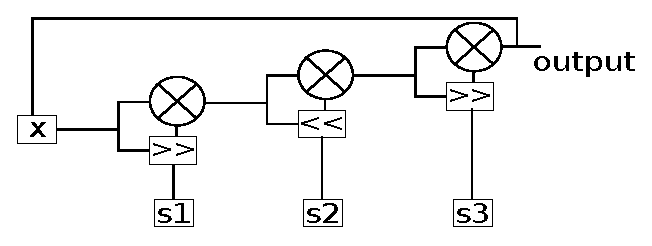
\includegraphics[width=6.5cm]{xorshift.eps}
  \label{xorshift verilog}}
  \subfigure[BBS]{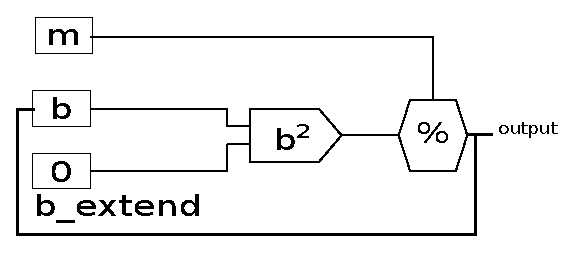
\includegraphics[width=6.5cm]{bbs.eps}
  \label{BBS verilog}}
  \subfigure[The proposed CIPRNG]{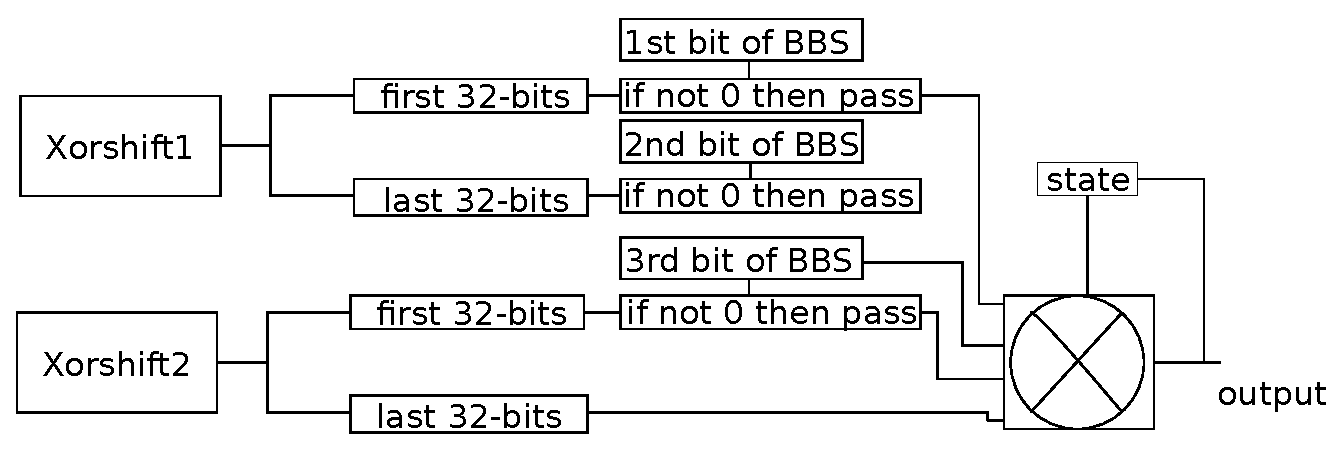
\includegraphics[width=10cm]{ci.eps}
  \label{CI verilog}}
\end{center}
\caption{The processing structure for BBS in FPGA (per clock step)}
\end{figure}
%In our program, we define 
%each FPGA clock positive edge, the XORshift will work, since these are simple processing for FPGA, every 
%clock step can lead to one output.

\subsection{Design of BBS}
Fig.\ref{BBS verilog} gives the proposed design of the BBS generator in FPGAs.
There are two inputs of $32$ bits, namely 
$b$ and $m$. 
Register $b$ stores the state of the system
at each time (after the square computation). 
$m$ is also a register that saves the value of $M$, which must not change.
Another register $b\_extend$ 
is used to combine $b$ to a data having $64$ bits, with a view to avoid overflow. 
After the last computation,
the three LSBs from the output of $\%$ are
taken as output. 
Let us notice that a BBS is
 performed at each time unit.

\begin{figure}
\begin{center}
  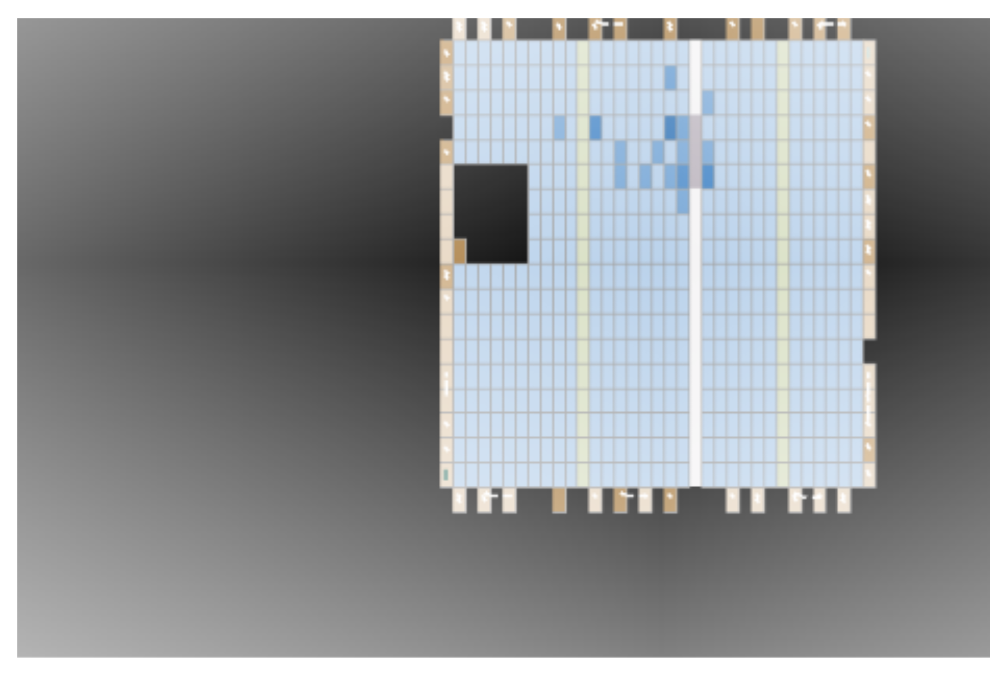
\includegraphics[width=6.5cm]{print.eps}
\end{center}
\caption{The sources cost in $EP2C8Q208C8$ FPGA board}
 \label{logic elements}
\end{figure}

\subsection{Design of the chaotic iterations}
Two XORshifts and one BBS are connected to work together, in order to compose the
proposed CIPRNG (see Fig.\ref{CI verilog}). 
As it can be shown, the three bits of the BBS output are switches for the corresponding $32$ bits XORshift outputs. Every round of the 
 processing costs two time units
 to be performed: in the first clock, 
the four PRNGs are processed in parallel,
whereas in the second one, the results of these generators are combined with 
the current state of the system, in order to produce the output of $32$ bits. 

In our experiments, the type $EP2C8Q208C8$ from Altera 
company's CYCLONE II FPGA series 
has been used. By default, its working
frequency is equal to $50$ MHz.
However, it is possible to increase it until
$400$ MHz by using the phase-lock loop (PLL) device.
In that situation, the CIPRNG designed on this
FPGA can produce about $6400$ Mbits per second
(that is, $400 (MHz) \div 2 (times) \times 32 (bits)$),
while using $3652$ of the $8256$ logic 
elements in $EP2C8Q208C8$ (see
Fig.\ref{logic elements}). 

In the next section, an application of this 
CSPRNG designed on FPGA in the information 
hiding security fields is detailed, to show
that this hardware pseudorandom generator 
is ready to use.
